\textbf{Theorem 6 makes a prediction about the geometric rate of convergence in the third pane of Output 12. Exactly what is this prediction? How well does it match the observed rate of convergence?}
\newline


Since $f(x) = \frac{1}{1+x^2}$ is analytic everywhere exept $x=\pm i$, where it has singularities, it is analytic on and inside the ellipse with foci $\{-1,1\}$ and semiminor axis $b < 1$ on which the Chebishev potential takes the value
\begin{align*}
\phi_f = \log\left(\frac{1}{2}(a+b)\right) \approx \log\left(\frac{1}{2}(\sqrt{2}+1)\right),
\end{align*}
where we have obtained a from the foci identity $ f = a^2 - b^2$. Hence, by \textsc{Theorem 6}, the convergence should be
\begin{align*}
|w_j-u^{(v)}(x_j)| = \mathcal{O}\left(e^{-N(\phi_f+\log{2})}\right) = \mathcal{O}\left(e^{-(\sqrt{2}+1)N}\right),
\end{align*}
which is proved to be right by the next figure.
\begin{figure}[H]
\centering
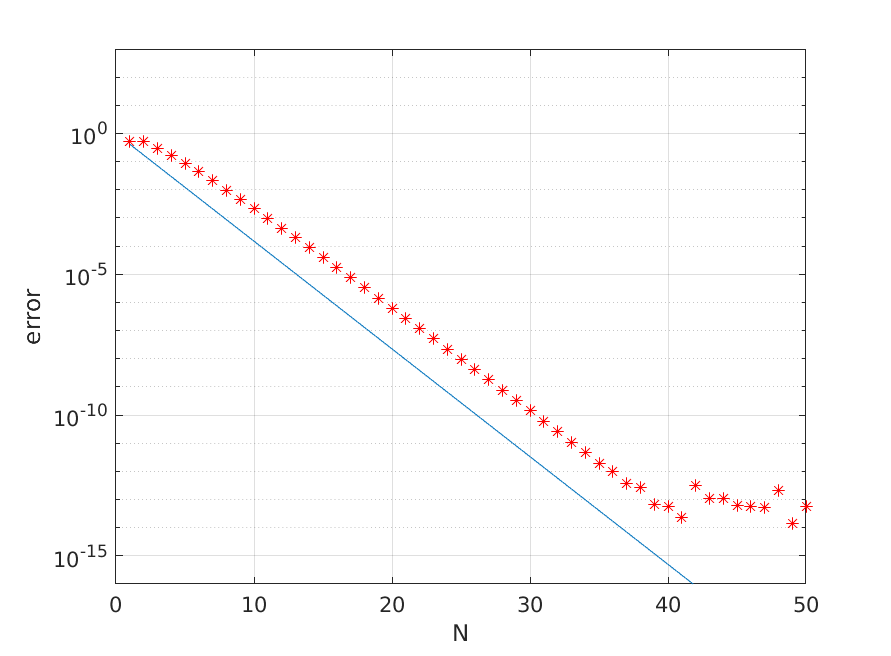
\includegraphics[scale=0.75]{P6_7.png}\caption{Acuracy of the Chebishev spectral derivative for $f(x) = \frac{1}{1+x^2}$.}
\end{figure}

\subsection*{Matlab code for this problem}
\begin{verbatim}
%% Problem 3 - 6.7 Trefethen
Nmax = 50; E = zeros(Nmax,1);
for N = 1:Nmax
    [D,x] = cheb(N);
    v = 1./(1+x.^2); vprime = -2*x.*v.^2;    % analytic in [-1,1]
    E(N) = norm(D*v-vprime,inf);
end
% Define ellipse and potential on it.
a = sqrt(2) ; b = 1;
phif = log(0.5*(a+b));
% Plot results:
figure
semilogy(1:Nmax,E(:),'r*')
hold on
semilogy(1:Nmax,exp(-(phif+log(2))*(1:Nmax)))
axis([0 Nmax 1e-16 1e3]), grid on
set(gca,'xtick',0:10:Nmax,'ytick',(10).^(-15:5:0))
xlabel N, ylabel error
txt='Latex/FIGURES\P6_7';
saveas(gcf,txt,figformat)
\end{verbatim}
